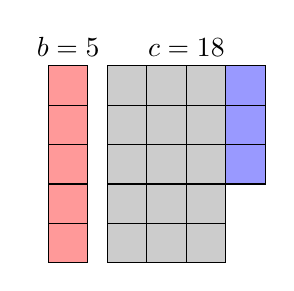
\begin{tikzpicture}[scale=0.5]
  % Parameters
  \def\a{18}     % total number
  \def\b{5}      % divisor
  \pgfmathsetmacro{\q}{int(\a/\b)} % quotient
  \pgfmathsetmacro{\r}{mod(\a,\b)} % remainder

  % Draw squares
  \foreach \i in {0,...,\numexpr\a-1} {
    \pgfmathtruncatemacro{\col}{int(\i/\b)}
    \pgfmathtruncatemacro{\row}{int(mod(\i,\b))}
    \ifnum\col=\q
    \draw[fill=blue!40] (\col, -\row) rectangle ++(1, -1); % remainder
    \else
    \draw[fill=black!20] (\col, -\row) rectangle ++(1, -1); % full blocks
    \fi
  }

  \foreach \i in {0,...,\numexpr\b-1} {
    \draw[fill=red!40] (-1.5, -\i) rectangle ++(1, -1);
  }

  \path (-1.5, 0) -- ++(1, 0) node[midway, above] {$b = \b$};
  \path (0, 0) -- ++(\q+1, 0) node[midway, above] {$c = \a$};
\end{tikzpicture}

